\chapter{Realizability}
\label{chap:realizability}

\section{Basic definitions}
\label{sec:basic-definitions}

\subsection{Motivation and the basic idea}
\label{sec:realizability-basic-idea}

Realizability was introduced by Stephen Kleene~\sidecite{KleeneSC:intint}
who used it to build a model of intuitionistic arithmetic. Our purpose
is to study not only the theoretical aspects of computable
mathematics, but also practical issues. Thus we approach realizability
by asking a practical question: given a mathematical structure
(constants, functions, relations, and axioms), what should a computer
implementation look like? For simple cases, the answer is obvious. A
group would have a type whose values represent group elements, a value
representing the neutral element, and functions which compute the
group operation and inverses. But for more interesting structures,
especially those arising in mathematical analysis, the answer is less
clear. How do we implement the real numbers (and we do not mean
floating-point arithmetic, we mean the \emph{real} real numbers)?
Which operations on a compact metric space can be implemented? How do
we implement a space of smooth functions? Significant research goes
into finding satisfactory answers to such
questions~\sidecite{Wei00,TZ98,Bla97}.

To explain the basic idea behind realizability we consider a small
real-world programming example. Suppose we are asked to design a data
structure for the set $\mathsf{Graphs}$ of all finite
simple\sidenote{Simple means at most one arrow between any two
  vertices.} directed graphs with vertices labeled by distinct
integers. A typical graph~$G$ is shown in Figure~\ref{fig:digraph}.

\begin{figure}[htp]
  \centering
  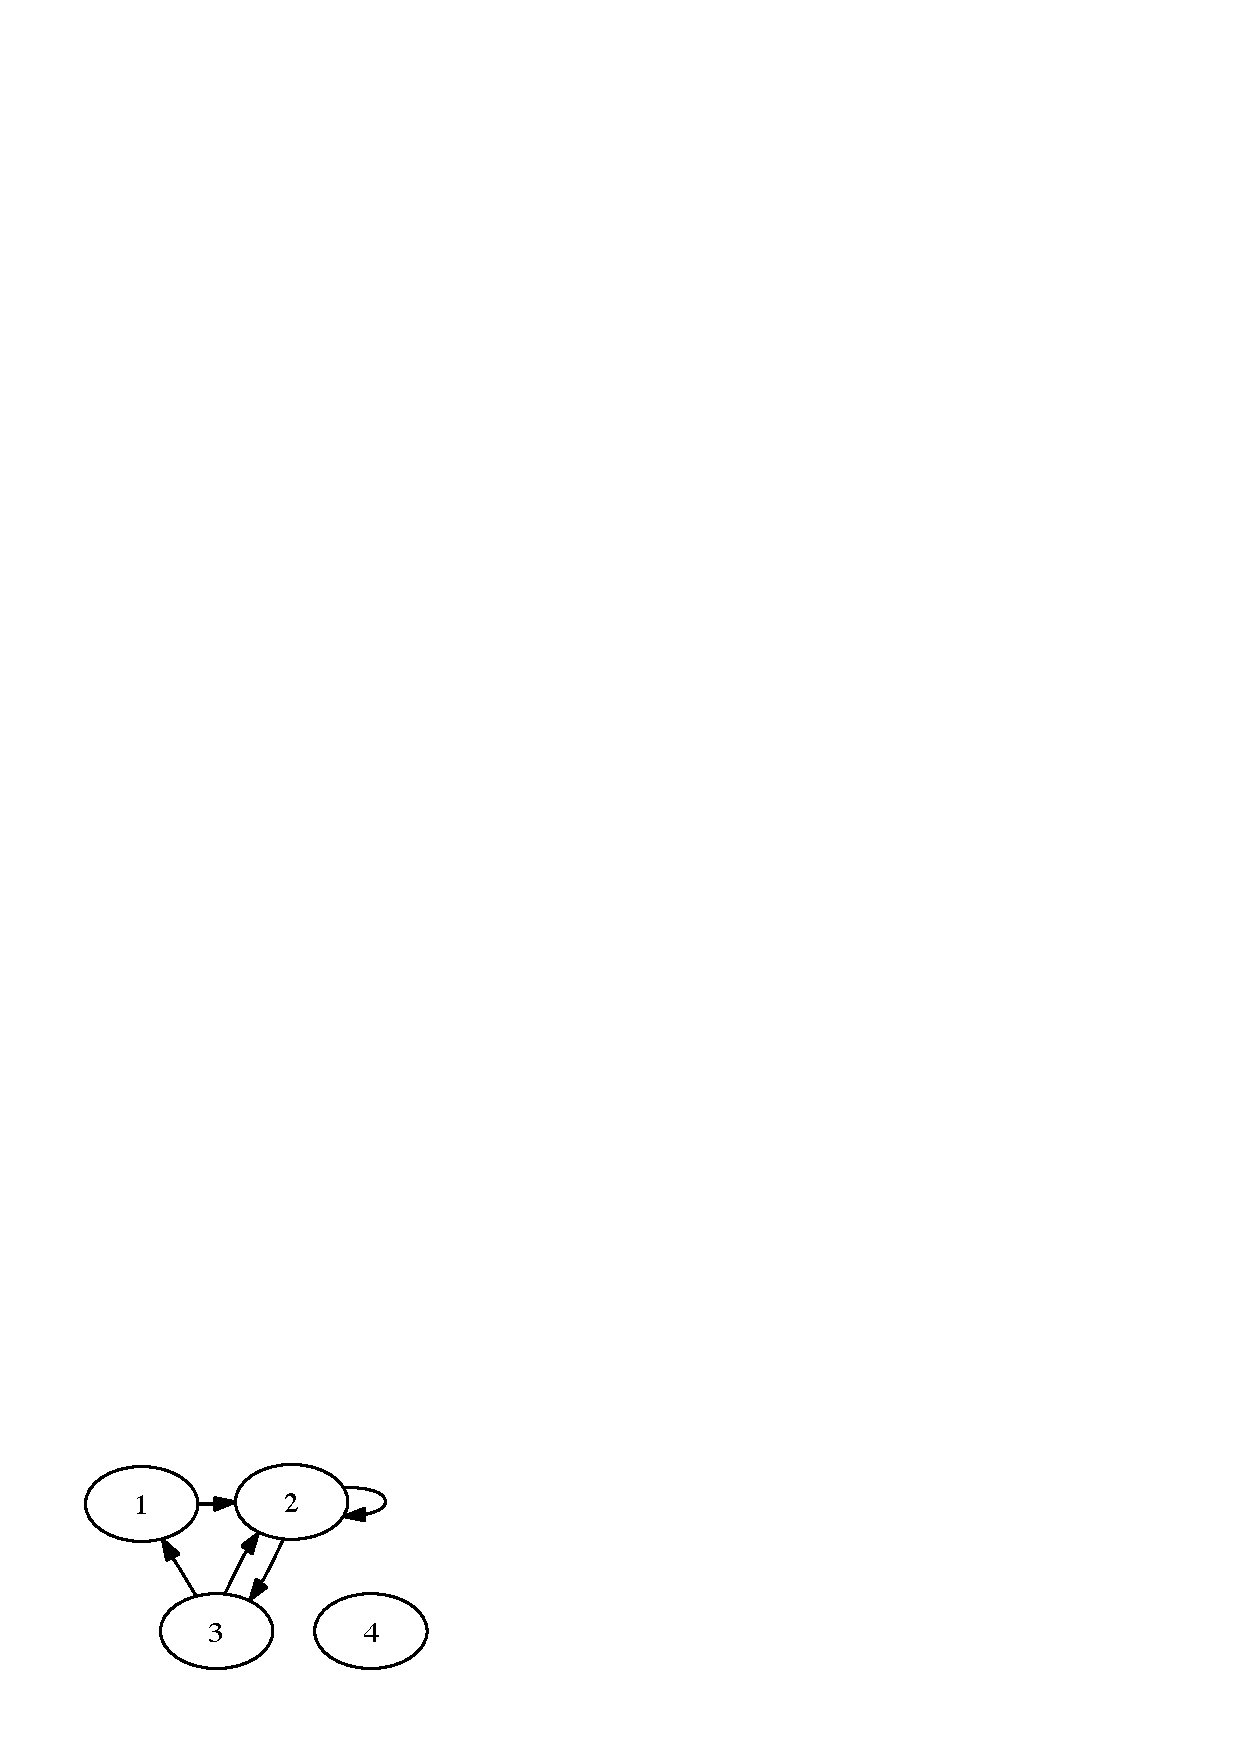
\includegraphics[width=0.3\textwidth]{digraph}
  \caption{A finite directed graph $G$}
  \label{fig:digraph}
\end{figure}

One common representation of such graphs uses a pair of lists
$(\ell_V, \ell_A)$, where $\ell_V$ is the list of vertex labels and
$\ell_A$ is the \emph{adjacency list} representing the arrows by
pairing the labels of each source and target. For the above graph $G$,
$\ell_V = [1, 2, 3, 4]$ and $\ell_A = [(1,2), (2,2), (2,3), (3,2),
(3,1)]$.
%
Thus we define the datatype of graphs as\sidenote{We use Haskell
  notation in which $[t]$ is the type of lists of elements of
  type~$t$, and $(t_1, t_2)$ is the cartesian product of types~$t_1$
  and~$t_2$.}
%
\begin{lstlisting}[language=Haskell]
type Graph = ([Int], [(Int, Int)])
\end{lstlisting}
%
However, this is not a complete description of the intended
representation, as there are representation invariants and conditions
not expressed by the type, e.g.,
%
\begin{enumerate}
\item The order in which vertices and arrows are listed is not
  important%
; for example, $[1,2,3,4]$ and $[4,1,2,3]$ represent the same vertices.
\item Each vertex and arrow must be listed exactly once.
\item The source and target of each arrow must appear in the list of vertices.
\end{enumerate}
%
Consequently, to fully implement the mathematical
set~$\mathsf{Graphs}$ we must not only decide on the underlying
datatype $\mathtt{graph}$, but also determine what values of that type
represent which elements of~$\mathsf{Graphs}$. All this can be
expressed with a \defemph{realizability relation}
%
\begin{equation*}
  r \rz x
\end{equation*}
%
which is read as ``datum~$r$ realizes (or implements, or represents)
element~$x$''. In the above example we would write
%
\begin{equation*}
([1, 2, 3, 4], [(1,2), (2,2), (2,3), (3,2), (3,1)]) \rz G.
\end{equation*}
%
Once the set $\mathsf{Graphs}$ is implemented as a datatype, an
obvious thing to do is to compute with it. When can we say that a
function $f : \mathsf{Graphs} \to \mathsf{Graphs}$ is computable? The
answer again is quite natural for a programmer: $f$ is computed by a
program $p : \mathtt{graph} \to \mathtt{graph}$ when $p$ does to
realizers what $f$ does to elements: if $r \rz G$ then $p \; r \rz
f(G)$. We say that the map $f$ is \defemph{realized} or \defemph{tracked} by
the program~$p$.

We adopt the notational convention that a realizer for an element or a
function is denoted by the same letter in fixed-width font. Thus
realizers for $x$, $y$, $f$, $g$ are denoted by $\R{x}$, $\R{y}$,
$\R{f}$, $\R{g}$, respectively.

\subsection{Assemblies}
\label{sec:assemblies}

We now give a precise definition of the ideas presented in the
previous section.

\begin{definition}[Assemblies]
  Let $\AA$ be a TPCA and $\compAA$ a sub-TPCA. An \defemph{assembly}
  over~$(\AA, \compAA)$ is a triple $\asm{S} = \xasm{S}$ where $S$ is
  a set, $|S|$ is a type, and $\rz_S$ is a relation between
  $\xAtyp{S}$ and~$S$ satisfying: for every $x \in S$ there is $\R{x}
  \in \xAtyp{S}$ such that $\R{x} \rz_S x$.

  A \defemph{realized map} $f : \asm{S} \to \asm{T}$ between assemblies
  $\asm{S}$ and $\asm{T}$ is a map $f : S \to T$ between the
  underlying sets for which there exists $\R{f} \in \compAtyp{|S| \to
    |T|}$ satisfying: if $\R{x} \rz_S x$ then $\defined{\R{f} \cdot
    \R{x}}$ and $\R{f} \cdot \R{x} \rz_T f(x)$.
\end{definition}

There are many versions of realizability. Ours is known as \emph{typed
  relative realizability}. It is typed because we used typed PCAs
rather than the ordinary ones. It is relative because we used one
TPCA~$\AA$ for assemblies, and another for the realized maps. By this we
are capturing the idea that computable functions may operate on
potentially non-computable data, as was the case for type~2 machines
and the graph model, cf.\ Sections~\ref{sec:type-2}
and~\ref{sec:graph-model}. In the typical case the larger TPCA~$\AA$
allows representation of arbitrary data, but the sub-TPCA $\compAA$
consists only of the computable part of~$\AA$ which forces the realizers
for maps to be computable. Thus it makes sense to say in the general
case that the maps are realized \emph{relative} to the choice of a
sub-TPCA~$\compAA$.

When $\AA$ is not typed the definition of an assembly simplifies a bit
because we need not keep mentioning the (trivial) types: an assembly
over a PCA~$\AA$ is a pair $(S, {\rz_S})$ where $S$ is a set and $\rz_S$
is a relation between~$\AA$ and~$S$, such that for every $x \in S$ there
is $r \in A$ and $r \rz_S x$.

Another special case occurs when $\compAA = \AA$. In this case we write
$\Asm{\AA}$ instead of $\Asm{\AA,\AA}$.

In most examples the TPCA $\AA$ is actually an NR-TPCA, and $\compAA$ a
sub-NR-TPCA of~$\AA$.

\begin{proposition}
  Assemblies and realized maps form the \defemph{category $\AsmA$ of
    assemblies over $(\AA, \compAA)$}.
\end{proposition}

\begin{proof}
  If $f : \asm{S} \to \asm{T}$ and $g : \asm{T} \to \asm{U}$ are
  realized by $\R{f} \in \compAtyp{|S| \to |T|}$ and $\R{g} \in
  \compAtyp{|T| \to |U|}$, respectively, then their composition $g
  \circ f$ is realized by $\pcalam{\annot{x}{|S|}}{r\;(q\;x)} =
  \combS\;(\combK\;r)\;(\combS\;(\combK\;q)\;(\combS\;\combK\;\combK))$.
  The identity map $\id_S : \asm{S} \to \asm{S}$ is realized by
  $\pcalam{\annot{x}{|S|}}{x} = \combS\;\combK\;\combK$. Composition
  is associative because it is just composition of maps.
\end{proof}

A common way to get isomorphic assemblies is the following.

\begin{lemma}
  \label{lemma:iso-assembly}
  %
  Suppose $\asm{S}$ is an assembly, $T$ is a set, and $f : T \to S$ is
  a bijection. Then $\asm{S}$ is isomorphic to $\asm{T} = (T, |S|,
  {\rz_T})$ where $r \rz_T x$ is defined as $r \rz_S f(x)$.
\end{lemma}

\begin{proof}
  The map $f$ is a morphism from $\asm{S}$ to $\asm{T}$ because it is
  tracked by~$\pcalam{\annot{x}{|S|}}{x}$. Similarly, $\inv{f}$ is a
  morphism because it is also tracked by the same realizer. Obviously,
  $f$ and $\inv{f}$ are inverses of each other.
\end{proof}


\subsection{Modest sets}
\label{sec:modest-sets}

Suppose $\asm{S}$ is an assembly over $(\AA, \compAA)$. The only
requirement for the realizability relation $\rz_S$ is that every $x
\in S$ be realized by some $r \in \xAtyp{S}$. In particular, different
elements $x, y \in S$ may share the same realizer $r \in \xAtyp{S}$.
It is often reasonable to prohibit such anomalies.

\begin{definition}
  An assembly $\asm{S}$ is \defemph{modest} when each $r \in \xAtyp{S}$
  realizes at most one element of~$S$. A modest assembly is also
  called a \defemph{modest set}.
\end{definition}

\noindent
In symbols, modesty is the property
%
\begin{equation*}
  \all{r}{\xAtyp{S}}{
    \all{x,y \in S}
      (r \rz_S x \land r \rz_S y \implies x = y)
  }.
\end{equation*}
%
The full subcategory of $\Asm{A,\comp{A}}$ of the modest sets is
denoted by~$\Mod{\AA, \compAA}$. The terminology was suggested by Dana
Scott~\sidecite{Scott:modest-sets}, and modesty refers to the fact that
the cardinality of a modest~$S$ set does not exceed the cardinality of
$\xAtyp{S}$.

Most structures in computable mathematics turn out to be modest.
However, sometimes assemblies are needed, especially when we talk
about multi-valued maps and hyperspaces,
cf.~Sections~\ref{sec:multi-valued-functions}
and~\ref{sec:hyperspaces}.


\subsection{Constant assemblies}
\label{sec:nabla}

The extreme case of elements sharing the same realizer happens when
all elements of a set share all realizers. Assemblies with this
property are called \defemph{constant assemblies}. They give us a way of
representing arbitrary sets.

Let $t$ be a type such that $\Atyp{t}$ is inhabited. Such a type
always exists, because there is at least one type $s$, and then
$\Atyp{s \to s \to s}$ contains $\combK_{s,s}$. Given any set $X$, let
$\nabla X = (X, t, {\rz_{\nabla X}})$ be the assembly whose underlying
set is~$X$ and the realizability relation is trivial, i.e., $r
\rz_{\nabla X} x$ for all $x \in X$ and $r \in A_t$. If $f : X \to Y$
is any map between sets~$X$ and~$Y$ then~$f$ is a morphism $\nabla f :
\nabla X \to \nabla Y$ because it is tracked by
$\pcalam{\annot{x}{t}}{x}$. This defines a functor
%
\begin{equation*}
  \nabla : \Set \to \AsmA.
\end{equation*}
%
Up to natural isomorphism, $\nabla$ is independent of the choice of
type~$t$. We will study the properties of $\nabla$ later on. For now
we notice that $\nabla$ is full and faithful, which means that
$\AsmA$ contains the category of sets as a full
subcategory.

The functor $\nabla$ is devoid of any computational content because it
represents a set~$X$ by a trivial realizability relation which conveys
no information at all about the elements of~$X$. Consequently, from
the realizers we cannot compute anything interesting regarding~$X$.


\section{Equivalent formulations}
\label{sec:equivalent-formulations}

Assemblies and modest sets have several equivalent formulations, which
were formulated by different communities for particular choices of
$(\AA, \compAA)$. Consequently, different people prefer to work with
different formulations of realizability, and use their own notation
and terminology. In this section we review the equivalent
formulations, and in the next one the popular ``schools'' of
computability.

\subsection{Existence predicates}
\label{sec:existence-predicates}

A realizability relation $\rz_S$, which is a subset of $\xAtyp{S}
\times S$, may be equivalently expressed as a map $\Ex_S : S \to
\pow{\xAtyp{S}}$. The correspondence is
%
\begin{equation*}
  \R{x} \rz_S x \iff \R{x} \in \Ex_S(x).
\end{equation*}
%
Because every $x$ is realized by something, $\Ex_S(x)$ always contains
at least one element. Thus an assembly $\xasm{S}$ may be equivalently
presented as a triple $(S, |S|, \Ex_S)$ where $\Ex_S : S \to
\pow{\xAtyp{S}}$ is a map such that $\Ex_S(x)$ contains at least one
element for every $x \in S$. The map $\Ex_S$ is called \defemph{existence
  predicate} because we can think of the realizers $\Ex_S(x)$ as
computational witnesses for ``existence of~$x$''.

An assembly $S$ is modest if, and only if, $\Ex_S(x) \cap \Ex_S(y)
\neq \emptyset$ implies $x = y$.

Under this formulation a map $f : \asm{S} \to \asm{T}$ is realized if
there exists $\R{f} \in \compAtyp{|S| \to |T|}$ such that, for all $x
\in S$ and $\R{x} \in \Ex_S(x)$, $\defined{\R{f}\;\R{x}}$ and
$\R{f}\;\R{x} \in \Ex_T(f(x))$.

\subsection{Representations}
\label{sec:representations}

By turning the existence predicate around we obtain
\defemph{representations}. Suppose first that $S$ is a modest set. Since
every realizer $r \in \xAtyp{S}$ realizes at most one $x \in S$, we may
define a partial map $\delta_S : \xAtyp{S} \parto S$ by
%
\begin{equation*}
  \delta_S(x) = r \iff r \rz_S x.
\end{equation*}
%
The map $\delta_S$ is surjective because every $x \in S$ is realized,
but it need not be defined everywhere. The triple $(S, |S|, \delta_S)$
uniquely describes the modest set~$S$. The map $\delta_S$ is called a
\defemph{representation} of~$S$.

A map $f : S \to T$ is realized or tracked by $\R{f} \in \compAtyp{|S|
  \to |T|}$ when, for all $\R{x} \in \dom{\delta_S}$,
$\defined{\R{f}\;\R{x}}$ and $\delta_T(\R{f}\;\R{x}) =
f(\delta_S(x))$.

The category of representations and realized maps is denoted
by~$\Rep{\AA,\compAA}$. It is of course equivalent to $\Mod{\AA,
  \compAA}$, but sometimes we want to make the distinction and so we
give it a symbol.

A general assembly $\asm{S}$ may also be expressed as a
representation, if we allow $\delta_S$ to be a multi-valued partial
surjection $\delta_S : \xAtyp{S} \multito S$. The relationship between
the realizability relation $\rz_S$, the existence predicate $\Ex_s$
and the representation $\delta_S$ is
%
\begin{equation*}
  r \rz_S x \iff
  r \in \Ex_S(x) \iff
  x \in \delta_S(r).
\end{equation*}


\subsection{Partial equivalence relations}
\label{sec:pers}

This formulation only works for modest sets, not for general
assemblies. With each modest set~$S$ we may associate a partial
equivalence relation (per)\sidenote{A partial equivalence relation is
  a relation which is transitive and antisymmetric.} $\per_S$ on
$\xAtyp{S}$ which relates~$q$ and~$r$ when they realize the same
element:
%
\begin{equation*}
  q \per_S r \iff
  \some{x}{S}{q \rz_S x \land r \rz_S x}.
\end{equation*}
%
The pair $(|S|, {\per_S})$ suffices for the reconstruction of the
original modest set, up to isomorphism. Let us be a bit more precise
about this.

Let $\AA$ be a TPCA and $\comp{A}$ a sub-TPCA. A \defemph{partial
  equivalence relation} on~$\AA$ is a pair $S = (|S|, {\per_S})$ where
$|S|$ is a type and $\per_S$ is a transitive and antisymmetric
relation on $\xAtyp{S}$. A realizer $r \in \xAtyp{S}$ is \defemph{total} if
$r \per_S r$. The set of total realizers is denoted by $\|S\| = \set{r
  \in \xAtyp{S} \such r \per_S r}$. Each $r \in \|S\|$ is a member of
its equivalence class $[r]_S = \set{q \in \xAtyp{S} \such r \per_S q}$.

An \defemph{extensional realizer} between pers $S$ and $T$ is $p \in
\compAtyp{|S| \to |T|}$ such that, for all $q, r \in \xAtyp{S}$, if $q
\per_S r$ then $\defined{p\;q}$, $\defined{p\;r}$, and $p\;q \per_T
p\;r$. Extensional realizers $p$ and $p'$ are \defemph{equivalent} when
$q \per_S r$ implies $p\;q \per_T p'\;r$.

Pers and equivalence classes of extensional realizers form a category
$\Per{\AA, \compAA}$ whose objects are pers on~$\AA$ and morphisms are
equivalence classes of extensional realizers. The composition of $[p]
: S \to T$ and $[q] : T \to U$ is $[q \circ p] : S \to U$ where $q
\circ p = \pcalam{\annot{x}{|S|}}{q\;(p\;x)}$. The identity morphism
$\id_S : S \to S$ is represented by $\xpcalam{\annot{x}{|S|}}{x}$. It
is easy to check that this forms a category.

Let $S$ and $T$ be pers over $(\AA, \compAA)$. A morphism between them
may be alternatively described as a function $f : \|S\|/{\per_S} \to
\|T\|/{\per_T}$ between the equivalence classes for which there exists
a realizer $p \in \compAtyp{|S| \to |T|}$ that tracks it: for every
equivalence class $[r]_S$, $\defined{p\;r}$ and $[p\;r]_T = f([r]_S)$.

\begin{proposition}
  The categories $\Mod{\AA, \compAA}$ and $\Per{\AA, \compAA}$ are
  equivalent.
\end{proposition}

\begin{proof}
  A modest set $\xasm{S}$ determines a per $(S, {\per_S})$,
  as described above. A morphism $f : S \to T$ which is tracked by $p
  \in \compAtyp{|S| \to |T|}$ determines a morphism of pers $[p] : (S,
  {\per_S}) \to (T, {\per_T})$. This defines a functor $F : \Mod{\AA,
    \compAA} \to \Per{\AA, \compAA}$.

  In the other direction the functor $G : \Per{\AA, \compAA} \to
  \Mod{\AA, \compAA}$ sends a per $(|T|, {\per_T})$ to the modest set
  $(\|T\|/{\per_T}, |T|, {\rz_T})$ whose realizability relation is
  %
  \begin{equation*}
    r \rz_T [q] \iff r \per_T q.
  \end{equation*}
  %
  A morphism $[p] : (S, {\per_S}) \to (T, {\per_T})$ is mapped to the
  map $G [p] : \|S\|/{\per_S} \to \|T\|/{\per_T}$, defined by $G [p]
  [r]_S = [p\;r]_T$, which is obviously tracked by~$p$.

  The functors $F$ and $G$ form an equivalence of categories. The
  composition $F \circ G$ is actually equal to identity, as is easily
  verified. A modest set~$\xasm{S}$ is isomorphic to
  $G(F(S))$ by Lemma~\ref{lemma:iso-assembly} applied to the bijection
  which takes an $x \in S$ to $[r]_{G(F(S))}$, where $r \in \xAtyp{S}$
  is any realizer such that $r \rz_S x$. We leave the verification
  that the isomorphisms are natural as exercise.
\end{proof}


\subsection{Equivalence relations}
\label{sec:ers}

A per $(|S|, {\per_S})$ may be viewed as an equivalence relation on
$\|S\| = \set{r \in \xAtyp{S} \such r \per_S r}$. This gives us yet
another equivalent formulation of modest sets, this time in terms of
equivalence relations.

Let us state explicitly what the category $\Er{\AA, \compAA}$ of
equivalence relations is. The objects are triples $(S, |S|,
{\equiv_S})$ where $|S|$ is a type, $S \subseteq \xAtyp{S}$, and
$\equiv_S$ is an equivalence relation on~$S$. As in the case of pers,
a morphism $(S, |S|, {\equiv_S}) \to (T, |T|, {\equiv_T})$ is
represented by an extensional realizer $p \in \compAtyp{|S| \to |T|}$.

The difference between pers and equivalence relations is mostly a
bureaucratic one. Nevertheless, it is useful to know about $\Er{\AA,
  \compAA}$ because sometimes we can describe it in useful
alternative ways, e.g., in Section~\ref{sec:equilogical-spaces} we
describe pers on the graph model as equivalence relations on
topological spaces.


\section{Schools of Computable Mathematics}
\label{sec:schools}

Computable mathematics was developed by several ``schools'', mostly
independent of each other, and each coming from its own tradition.
Realizability covers most approaches to computable mathematics that
have been proposed. To get a particular variation we just choose an
appropriate TPCA with sub-TPCA. We look at some of them and relate the
traditional terminology and notions to ours.

\subsection{Recursive Mathematics}
\label{sec:recursive-math}

\emph{Recursive Mathematics}~\sidecite{type-1}, also known as \emph{type
  one effectivity} or \emph{Russian constructivism}~\sidecite{russ}, is
computable mathematics done with type 1 machines, cf.\
Section~\ref{sec:type-1}. In our settings it corresponds to the
category $\Rep{\NN}$ of representations over the first Kleene algebra.

An object of $\Rep{\NN}$ is called a \defemph{numbered set}. It is a pair
$(S, \delta_S)$, where $S$ is a set $\delta_S : \NN \parto S$ a
partial surjection, called a \defemph{numbering} of~$S$. A function $f :
S \to T$ is \defemph{realized} by $n \in \NN$ when, for all $m \in
\dom{\delta_S}$,
%
\begin{equation*}
  \text{$\defined{\pr{n}{m}}$ and $\delta_T(\pr{n}{m}) = f(\delta_S(m))$.}
\end{equation*}
%
A numbered set $(S, \delta_S)$ has countably many elements because it
is covered by the countable set~$\dom{\delta_S}$. This is sometimes
considered a disadvantage and a reason for preferring type~2 machines,
which are able to compute with uncountable structures such as real
numbers. However, in Section~\ref{countable-sets} we will see that a
numbered set may be \emph{internally uncountable}, i.e., it appears to
be uncountable inside the category of numbered sets. In fact, it is
perfectly possible to develop analysis in this setting. One gets an
unusual variant which is a rich source of counter-examples.

\subsection{Equilogical spaces}
\label{sec:equilogical-spaces}

An equilogical space is a topological space with an
equivalence relation~\sidecite{BauerA:equs}. We study equilogical spaces
in some detail because they give us a general theory of computable
maps between countably-based spaces. In Section~\ref{sec:tte} we
relate equilogical spaces to Type Two Effectivity, which is another
school of computability on general topological spaces.

Recall that a topological space is \emph{countably-based} if it has a
countable topological basis. Equivalently, a space is countably-based
when it has a countable \emph{subbasis}. We prefer to work with
subbases because they simplify the treatment of computable maps
between spaces. Thus we define a countably-based space to be a pair
$(X, (U_i)_{i \in \NN})$ where $X$ is a topological space and
$(U_i)_{i \in \NN}$ is an enumeration of \emph{subbasic} open sets.
These generate the topology of $X$ by taking finite intersections and
arbitrary unions. While we usually omit an explicit mention of the
subbasis $(U_i)_{i \in \NN}$, we do insist that a countably-based
space always be given \emph{together with} a particular subbasis. This
allows us to avoid the axiom of choice.

The graph model~$\Scott$ is a countably-based space. We always take it
with the subbasis $(\upper{n})_{n \in \NN}$. Recall that $\upper{n} =
\set{A \subseteq \NN \such n \in A}$.

A \defemph{(countably-based) equilogical space} $(X, (U_i)_{i \in \NN},
{\equiv_X})$ is a countably-based topological space~$(X, (U_i)_{i \in
  \NN})$ with an equivalence relation~$\equiv_X$. We usually do not
bother writing the subbasis $(U_i)_{i \in \NN}$. The canonical
quotient map $q_X : X \to X/{\equiv_X}$ maps each $x \in X$ to its
equivalence class $[x]_X$. A morphism $f : (X,{\equiv_X}) \to
(Y,{\equiv_Y})$ is a map $f : X/{\equiv_X} \to Y/{\equiv_Y}$ between
equivalence classes for which there exists a continuous $g : X \to Y$
such that
%
\begin{equation*}
  \xymatrix@+1em{
    {X} \ar[d]_{q_X} \ar[r]^g
    &
    {Y} \ar[d]^{q_Y}
    \\
    {X/{\equiv_X}}
    \ar[r]_f
    &
    {Y/{\equiv_Y}}
  }
\end{equation*}
%
commutes, i.e., $f([x]_X) = [g(x)]_Y$ for all $x \in X$. Morphisms
compose as expected. The category of equilogical spaces and morphisms
between them is denoted by~$\Equ$.

A countably-based topological space $X$ may be construed as an
equilogical space $(X, {=_X})$ with equality as the equivalence
relation. A morphism $f : (X, {=_X}) \to (Y, {=_Y})$ is the same
thing as a continuous map $f : X \to Y$ so that we have a full and
faithful embedding $\wTop \to \Equ$ of the category $\wTop$ of
countably-based spaces into the category $\Equ$.

Let us show that $\Equ$ and $\Asm{\Scott}$ are equivalent. A
\defemph{pre-embedding} $e : X \to Y$ between topological spaces is a
continuous map such that $\inv{e} : \topol{Y} \to \topol{X}$ is
surjective. For $T_0$-spaces this is equivalent to~$e$ being an
embedding. If $(U_i)_{i \in I}$ is a topological subbasis for $Y$ and
$e : X \to Y$ is a pre-embedding, then $(\invim{e}(U_i))_{i \in I}$ is
a topological subbasis for~$X$.

\begin{theorem}[Embedding Theorem for $\Scott$]
  \label{thm:scott-embedding}%
  A space $X$ may be pre-emebedded in~$\Scott$ if, and only if, it is
  countably based.
\end{theorem}

\begin{proof}
  Here $\Scott$ is equipped with the Scott topology. If $e : X \to
  \Scott$ is a pre-embedding then the open sets $U_n =
  \invim{e}(\upper{n})$ form a countable subbasis for~$X$.

  Conversely, suppose $(U_n)_{n \in \NN}$ is a countable subbasis
  for~$X$. Define the map $e_X : X \to \Scott$ by
  %
  \begin{equation*}
    e_X(x) = \set{n \in \NN \such x \in U_n}.
  \end{equation*}
  %
  We claim that $e_X$ is a pre-embedding. It is continuous because
  $\invim{e_X}(\upper{n}) = U_n$. Let $V \subseteq X$ be open. Then 
  $V$ is a union of finite intersections of subbasic opens,
  %
  \begin{equation*}
    V = \tbigcup_i U_{n_{i,1}} \cap \cdots \cap U_{n_{i,k_i}}
  \end{equation*}
  %
  Now
  %
  \begin{align*}
    \invim{e_X}\left(\tbigcup_i \upper{\set{n_{i,1}, \ldots, n_{i,k_i}}}\right) &=
      \tbigcup_i \invim{e_X}(\upper{\set{n_{i,1}, \ldots, n_{i,k_i}}})
      \\
      &=
      \tbigcup_i \invim{e_X}(\upper{n_{i,1}} \cap \cdots \cap \upper{n_{i,k_i}})
      \\
      &=
      \tbigcup_i \invim{e_X}(\upper{n_{i,1}}) \cap \cdots \cap \invim{e_X}(\upper{n_{i,k_i}})
      \\
      &=
      \tbigcup_i U_{n_{i,1}} \cap \cdots \cap U_{n_{i,k_i}} \\
      &= V,
  \end{align*}
  %
  therefore $\invim{e_X}$ is surjective, as required.
\end{proof}

\noindent
%
The pre-embedding $e_X : X \to \Scott$ is called the \defemph{(subbasic)
  neighborhood filter} because $e_X(x)$ is just the set of (indices
of) subbasic neighborhoods of~$x$. Henceforth $e_X : X \to \Scott$
will always denote the subbasic neighobrhood filter.

\begin{theorem}[Extension Theorem for $\Scott$]
  \label{thm:scott-extension}%
  Suppose $e : X \to Y$ is a pre-embedding and $f : X \to \Scott$
  continuous. Then~$f$ has a continuous extension $g : Y \to \Scott$
  along~$e$.
\end{theorem}

\begin{proof}
  Consider the map $g : Y \to \Scott$ defined by
  %
  \begin{equation*}
    g(y) = \tbigcup_{U \in \topol{Y}} \left\{
      \tbigcap_{z \in \invim{e}(U)} f(z)
      \such
      y \in U
    \right\}.
  \end{equation*}
  %
  It is continuous because
  %
  \begin{align*}
    \invim{g}(\upper{n}) &=
    \set{y \in Y \such n \in g(y)} \\
    &=
    \set{y \in Y \such \some{U}{
        \topol{Y}}{y \in U \land
        \all{z}{\invim{e}(U)}{n \in f(z)}
      }
    } \\
    &=
    \tbigcup_{U \in \topol{Y}} \left\{
        U \such
        \all{z}{\invim{e}(U)}{n \in f(z)}
      \right\}.
  \end{align*}
  %
  Let us show that $g(e(x)) = f(x)$ for all $x \in X$. Consider the
  value
  %
  \begin{align*}
    g(e(x)) =
    \tbigcup_{U \in \topol{Y}} \left\{
      \tbigcap_{z \in \invim{e}(U)} f(z)
      \such
      e(x) \in U \right\}.
  \end{align*}
  %
  Because $f(x)$ appears in every intersection, each of them is
  contained in~$f(x)$, which shows that $g(e(x)) \subseteq f(x)$.
  Suppose $n \in f(x)$. Because $e$ is a pre-embedding there exists $W
  \in \topol{Y}$ such that $\invim{f}{\upper{n}} = \invim{e}(W)$. If
  $z \in X$ and $e(z) \in W$ then $z \in \invim{e}(W) =
  \invim{f}(\upper{n})$, hence $n \in f(z)$. The intersection
  $\tbigcap \left\{f(z) \such z \in X \land e(z) \in W \right\}$
  contains~$n$ and so $n \in g(e(x))$. We proved that $f(x) \subseteq
  g(e(x))$, therefore $f(x) = g(e(x))$.
\end{proof}

\noindent
%
The Embedding and Extension theorems now give us the desired
equivalence~\sidecite{Simpson-Menni}.

\begin{proposition}
  \label{prop:equ-equiv-asm-scott}%
  The categories $\Equ$ and $\Asm{\Scott}$ are equivalent.
\end{proposition}

\begin{proof}
  Suppose $(X, {\equiv_X})$ is an equilogical space, and let $e_X : X
  \to \Scott$ be the subbasic neighborhood filter pre-embedding.
  Define the assembly $F(X) = (X/{\equiv_X}, \Ex_{F(X)})$ by
  $\Ex_{F(x)} = \set{e_X(y) \such x \equiv_X y}$. To make $F$ into a
  functor we define $F(f) = f$ for a morphism $f : (X, {\equiv_X}) \to
  (Y, {\equiv_Y})$. If $f$ is tracked by $g : X \to Y$, then $F(f)$ is
  realized by a continuous extension of $e_Y \circ g : X \to \Scott$
  along~$e_X$, which exists by the Extension
  Theorem~\ref{thm:scott-extension}.

  The functor $G : \Asm{\Scott} \to \Equ$ is defined as follows. An
  assembly $(S, \Ex_S)$ is mapped to the equilogical space $G(S) =
  (X_S, \equiv_{G(S)})$ whose underlying space is the set $X_S =
  \set{(x,A) \in S \times \Scott \such A \in \Ex_S(x)}$, equipped with
  the unique topology that makes the projection $p : X_S \to \Scott$,
  $p : (x,A) \mapsto A$, a pre-embedding. Explicitly, the open subsets
  of $X_S$ are the inverse images $\invim{p}(U)$ of open subsets $U
  \subseteq \Scott$. Let $\equiv_{G(S)}$ be the equivalence relation
  defined by
  %
  \begin{equation*}
    (x,A) \equiv_{G(S)} (y,B) \iff x = y.
  \end{equation*}
  %
  A morphism $f : (S, {\rz_S}) \to (T, {\rz_T})$ which is tracked by
  $B \in \comp{\Scott}$ is mapped to $G(f) : X_S/{\equiv_{G(S)}} \to
  X_T/{\equiv_{G(T)}}$ defined by $G(f)([(x,A)]_{G(S)}) = [(f(x), B
  \cdot A)]_{G(T)}$.

  We leave the verification that $F$ and $G$ form an equivalence of
  categories as exercise.
\end{proof}

By restricting to the $T_0$-spaces we obtain another equivalence. Let
$\Equ_0$ be the full subcategory of~$\Equ$ in which the underlying
topological spaces are $T_0$-spaces.


\begin{proposition}
  \label{prop:equ0-equiv-mod-scott}
  The categories $\Equ_0$ and $\Mod{\Scott}$ are equivalent.
\end{proposition}

\begin{proof}
  We verify that the equivalence functors $F$ and $G$ from the proof
  of Proposition~\ref{prop:equ-equiv-asm-scott} restrict to $\Equ_0$
  and $\Mod{\Scott}$. If $(X, {\equiv_X})$ is an equilogical space
  whose underlying space $X$ is $T_0$, then the pre-embedding $e : X
  \to \Scott$ is actually an embedding. Because it is injective the
  assembly $F(X)$ is modest. This shows that $F$ restricts to a
  functor $\Equ_0 \to \Mod{\Scott}$.
  %
  To see that $G$ restricts to a functor $\Mod{\Scott} \to \Equ_0$,
  observe that, for a modest assembly $(S, \Ex_S)$, the projection
  $X_S \to \Scott$ is an embedding, therefore $X_S$ is a $T_0$-space.
\end{proof}

%%%%%%%%%%%%%%%%%%%%%%%%%%%%%%%%%%%%%%%%%%%%%%%%%%
\subsection{Computable countably-based spaces}
\label{sec:computable-countably-based-spaces}

We have so far studied the \emph{continuous} version of realizability
over the graph model in which the realizers for morphisms may be
arbitrary continuous maps. But what about the \emph{mixed}
version~$\Asm{\Scott, \comp{\Scott}}$, is it also equivalent to a
version of equilogical spaces? To see that the answer to the question
is affirmative, we first need to define computable maps between
countably-based spaces.

Recall from Section~\ref{sec:graph-model} that an enumeration operator
$g: \Scott \to \Scott$ is computable when its graph $\Gamma(g)$ is a
c.e.~set. By the Embedding Theorem~\ref{thm:scott-embedding}, every
countably based $T_0$-space $X$ can be embedded in $\Scott$, and every
continuous map $f: X \to Y$ can be extended to an enumeration operator
$g: \Scott \to \Scott$, so that the following diagram commutes:
%
\begin{equation*}
  \xymatrix{
    {X}   \ar@{ >->}[d]_{e_X} \ar[r]^f  &
    {Y} \ar@{ >->}[d]^{e_Y} \\
    {\Scott} \ar[r]^{g} &
    {\Scott}
  }
\end{equation*}
%
We can define a \defemph{computable continuous map} $f: X \to Y$ to be a
continuous map for which there exists a computable enumeration
operator $g: \Scott \to \Scott$ which makes the above diagram commute.
This idea gives the following definition of computable continuous
maps.

\begin{definition}
  \label{def:computable-map}%
  %
  \indexdef{computable continuous map}%
  %
  A continuous map $f : X \to Y$ between countably-based spaces $(X,
  (U_i)_{i \in \NN})$ and $(Y, (V_j)_{j \in \NN})$ is
  \defemph{computable} when there exists a c.e.~set $F \subseteq \NN
  \times \NN$ such that:
  %
  \begin{enumerate}
  \item
    %
    $F$ is monotone in the first argument: if $A \subseteq B \wayb
    \NN$ and $\pair{\code{A}, m} \in F$ then $(\code{B}, m) \in
    F$.
  \item
    %
    $F$ approximates~$f$: if $(\code{\set{i_1, \ldots, i_n}}, m) \in
    F$ then $f(U_{i_1} \cap \cdots \cap U_{i_n}) \subseteq V_m$.
  \item
    %
    $F$ converges to~$f$: if $f(x) \in V_m$ then there exist $i_1,
    \ldots, i_n$ such that $x \in U_{i_1} \cap \cdots \cap U_{i_n}$
    and $(\code{\set{i_1, \ldots, i_n}}, m) \in F$.
  \end{enumerate}
  %
  \indexdef{realizer!for computable continuous map}%
  %
  The relation~$F$ is called a~\defemph{c.e.~realizer} for~$f$. We also
  say that~$F$ \defemph{tracks}~$f$.
  %
  \indexdef{category!of effective topological spaces}%
  %
  The category of countably based spaces and computable continuous
  maps is denoted by $\compTop$.
\end{definition}

The category $\compTop$ is well-defined. The identity map $\id_X:
X \to X$ is tracked by the relation $I_X$, defined by
%
\begin{equation*}
  I_X = \set{
    (\code{\set{i_1, \ldots, i_n}}, m) \in \NN \times \NN \such
    m \in \set{i_1, \ldots, i_n}
  }.
\end{equation*}
%
The composition of computable maps $f: X \to Y$ and $g: Y \to Z$,
which are tracked by $F$ and $G$ respectively, is again a computable
map $g \circ f: X \to Z$ because it has a c.e.~realizer $H$ defined by
%
\begin{multline*}
  (\code{\set{j_1, \ldots, j_k}}, \ell) \in H
  \iff {} \\
    \some{i_1, \ldots, i_n}{\NN}{
      (\code{\set{i_1, \ldots, i_n}}, \ell) \in G \land
      \bigwedge\nolimits_{s = 1}^{n}
      (\code{\set{j_1, \ldots, j_k}}, i_s) \in F
    }.
\end{multline*}
%
The monotonicity condition in Definition~\ref{def:computable-map} is
redundant, for if $F$ is an c.e.~relation that satisfies the second
and the third condition, then we can recover monotonicity by defining
a new relation $F'$ by
%
\begin{equation*}
  F' = \set{(\code{A}, m) \in \NN \times \NN \such
    \bigvee\nolimits_{B \subseteq A} (\code{B}, m) \in F
  }.
\end{equation*}
%
It is easy to see that $F'$ satisfies all three conditions and
realizes the same function as~$f$.

A point $x \in X$ is \defemph{computable} when the map $\set{\star} \to
X$ which maps $\star$ to~$x$ is computable. This is equivalent to
requiring that $e_X(x) = \set{i \in \NN \such x \in U_i}$ is a
c.e.~set.

Next, we prove effective versions of the Embedding and Extension
Theorems.

\begin{theorem}[Computable Embedding Theorem]
  \label{th:computable_embedding_theorem}%
  %
  \index{Theorem!Computable Embedding Theorem}%
  \index{computable!Computable Embedding Theorem}%
  %
  Every countably-based space can be computably pre-embedded
  into~$\Scott$.
\end{theorem}

\begin{proof}
  We just need to provide a c.e.~realizer~$E_X$ for the neighborhood
  filter $e_X : X \to \Scott$. It is
  %
  \begin{equation*}
    E_X = \set{
      (\code{\set{i_1, \ldots, i_n}}, m) \in \NN \times \NN \such
      m \in \set{i_1, \ldots, i_n}
    }.
  \end{equation*}
  %
  This is obviously a c.e.~relation which is monotone in the first
  argument. The second condition for the c.e.~realizer~$E_X$ is
  %
  \begin{equation*}
     (\code{\set{i_0, \ldots, i_n}}, m) \in E_X
     \implies
     e_X(U_{i_1}, \ldots, U_{i_n}) \subseteq \upper{m},
  \end{equation*}
  %
  which clearly holds.
  %
  Suppose $e_X(x) \in \upper{m}$. Then $x \in U_m$, and
  $(\code{\set{m}}, m) \in E_X$, which proves the third condition.
\end{proof}

\begin{theorem}[Computable Extension Theorem]
  \label{th:computable_extension_theorem}%
  %
  \index{Theorem!Computable Extension Theorem}%
  \index{computable!Computable Extension Theorem}%
  %
  Let $X$ and $Y$ be countably-based topological spaces and $f: X \to
  Y$ a computable map between them. Then there exists a computable map
  $g: \Scott \to \Scott$ such that the following diagram commutes:
  %
  \begin{equation*}
    \xymatrix{
      {X} \ar[r]^{f} \ar@{ >->}[d]_{e_X}  &
      {Y} \ar@{ >->}[d]^{e_Y} \\
      {\Scott} \ar[r]_{g} &
      {\Scott} 
    }
  \end{equation*}
  %
\end{theorem}

\begin{proof}
  The maps $e_X$ and $e_Y$ are the computable embeddings from
  Theorem~\ref{th:computable_embedding_theorem}. Let $F$ be a
  c.e.~realizer for $f$. We define the map $g: \Scott \to \Scott$ by
  specifying its graph to be~$F$, i.e.,
  %
  \begin{equation*}
    g(A) = \set{m \in \NN \such
      \some{i_1, \ldots, i_n}{\NN}{
        (\code{\set{i_1, \ldots, i_n}}, m) \in F
      }}.
  \end{equation*}
  %
  All we have to show is that this choice of $g$ makes the diagram
  commute. For any $x \in X$,
  %
  \begin{align*}
    m \in g(e_X(x)) &\iff
      \some{i_1, \ldots, i_n}{\NN}{
        x \in U_{i_1} \cap \cdots \cap U_{i_n} \land
        (\code{\set{i_1, \ldots, i_n}}, m) \in F
      } \\
      &\iff
      f(x) \in V_m
      \\
      &\iff
      m \in e_Y(f(x)).
  \end{align*}
  %
  The second equivalence is implied from left to right by the second
  condition in Definition~\ref{def:computable-map}, and from right to
  the left by the third condition.
\end{proof}

We should point out that the computable continuous maps, as defined
here, work at the level of open sets, i.e., a c.e.~realizer $F$ for $f
: X \to Y$ operates on the (indices) of subbasic open sets. Therefore,
$F$ does not distinguish points that share the same neighborhoods,
even though $f$ might. This is not an issue with $T_0$-spaces in which
points are distinguished by their neighborhoods.


%%%%%%%%%%%%%%%%%%%%%%%%%%%%%%%%%%%%%%%%%%%%%%%%%%

\subsection{Computable equilogical spaces}
\label{sec:computable-equ}


With a notion of computable maps between spaces at hand, we can define
the computable equilogical spaces just like the ordinary ones, except
that we replace continuous maps by their computable versions.

\begin{definition}
  \label{def:computable-equ}%
  %
  \indexdef{computable!equilogical space}%
  \indexsee{computable!equilogical space}{equilogical space, comuptable}%
  \indexdef{equilogical space!computable}%
  %
  A morphism $f : (X, {\equiv_X}) \to (Y, {\equiv_Y})$ between
  equilogical spaces is \defemph{computable} if there exists a computable
  continuous map $g : X \to Y$ which tracks~$f$.
  %
  The category of equilogical spaces and computable morphisms between
  them is denoted by $\comp{\Equ}$.
\end{definition}

We check that we got the definition right by proving
that~$\comp{\Equ}$ is equivalent to $\Asm{\Scott, \comp{\Scott}}$.

\begin{proposition}
  \label{th:equivalence_compEqu_AsmScott}%
  %
  \index{equilogical space!computable!equivalent definitions}%
  %
  The categories $\Asm{\Scott, \comp{\Scott}}$ and $\comp{\Equ}$ are
  equivalent.
\end{proposition}

\begin{proof}
  The proof goes just as the proof of
  Propoistion~\ref{prop:equ-equiv-asm-scott} that $\Equ$ and
  $\Asm{\Scott}$ are equivalent. The only difference is that we refer
  to the Computable Embedding
  Theorem~\ref{th:computable_embedding_theorem} and the Computable
  Extension Theorem~\ref{th:computable_extension_theorem} in order to
  extend computable maps to computable enumeration operators.
\end{proof}

The category $\comp{\wTop}$ of countably-based spaces and computable
maps is embedded fully and faithfully into $\comp{\Equ}$. The
embedding works as in the continuous case: a topological space~$X$ is
mapped to the equilogical space $(X, {=_X})$, and a computable
continuous map $f : X \to Y$ is the same thing as a morphism $f : (X,
{=_X}) \to (Y, {=_Y})$.


%%%%%%%%%%%%%%%%%%%%%%%%%%%%%%%%%%%%%%%%%%%%%%%%%%
\subsection{Type Two Effectivity}
\label{sec:tte}

A popular realizability model is Kleene's~\sidecite{KV65} \defemph{function
  realizability}, which is better known by its newer name \defemph{Type
  Two Effectivity (TTE)}~\sidecite{Wei00}. As the names say, it is the
model of realizability based on functions and type 2 machines. 

TTE is traditionally expressed as a theory of representations. There
are actuallly three variations:
%
\begin{enumerate}
\item $\Rep{\Baire, \Baire}$ is the \emph{continuous} version in which
  maps are realized by continuous realizers.
\item $\Rep{\Baire, \comp{\Baire}}$ is the \emph{relative} version.
\item $\Rep{\comp{\Baire}, \comp{\Baire}}$ is the \emph{computable}
  version in which all realizers must be computable.
\end{enumerate}
%
Mostly only the first two of these are used. Sometimes multi-valued
representations are considered also, and for these we need to move to
the larger category of assemblies $\Asm{\Baire, \comp{\Baire}}$.

Specifically, a representation $(S, \delta_S)$ over the Baire space is
a partial surjection $\delta_S : \Baire \to S$. When $\delta_S(\alpha)
= x$ we say that $\alpha$ is a \defemph{$\delta_S$-name} of~$x$. A
\defemph{(continuously) realized map} $f :(S, \delta_S) \to (T,
\delta_T)$ is a map $f : S \to T$ for which there exists a partial
continuous map $g : \Baire \parto \Baire$ such that
$f(\delta_S(\alpha)) = \delta_T(g(\alpha))$ for all $\alpha \in
\dom{\delta_S}$. If the realizer $g$ is computable we say that $f$ is
\defemph{computably realized}. Recall that a computable $g$ corresponds
to a type~2 machine which converts a $\delta_S$-name of~$x$ to a
$\delta_T$-name of $f(x)$.

In the case of equilogical spaces there was a straightforward way of
turning a topological space into an equilogical space. The present
situation is less obvious. One obvious idea is to represent a
topological space~$X$ by a representation $\delta_X : \Baire \parto X$
for which $\delta_X$ is a quotient map. However, this is too weak a
requirement. To see this, suppose $\delta_X : \Baire \parto X$ and
$\delta_Y : \Baire \parto Y$ are representations of topological spaces
with $\delta_X$ and $\delta_Y$ topological quotient maps. Then a
continuous map $f : X \to Y$ may be lifted to $g : \Baire \parto Y$,
as in the diagram
%
\begin{equation*}
  \xymatrix@+1em{
    {\Baire}
    \ar[d]_{\delta_X}
    \ar[dr]^{g}
    \ar@{..>}[r]^{h?}
    &
    {\Baire}
    \ar[d]^{\delta_Y}
    \\
    {X}
    \ar[r]_f
    &
    {Y}
  }
\end{equation*}
%
because $\delta_X$ is a quotient map. But to make~$f$ into a morphism
we need a continuous realizer $h : \Baire \parto \Baire$ on the top
line, which however might not exist. A stronger property is required.

\begin{definition}
  Suppose $X$ is a topological space and $\delta_X : \Baire \parto X$
  is a representation and a topological quotient map. Then $\delta_X$
  is \defemph{admissible} if every continuous $g : \Baire \parto X$ has a
  continuous lifting $h : \Baire \parto \Baire$ such that
  $\delta_X(h(\alpha)) = g(\alpha)$ for all $\alpha \in \dom{g}$.
\end{definition}

Admissible representations are a central concept in TTE because they
are very well behaved. For example, if $\delta_X : \Baire \parto X$
and $\delta_Y : \Baire \parto Y$ are admissible, the continuous maps
$f : X \to Y$ coincide with the realized maps.

The spaces which have admissible representations have been studied in
depth~\sidecite{Schroeder,Weihrauch}. We only mention a basic result whose
proof is not too complicated.

\begin{proposition}
  Every countably-based $T_0$-space has an admissible representation.
\end{proposition}

\begin{proof}
  Suppose $(X, (U_i)_{i \in \NN})$ is a countably-based $T_0$-space,
  and let $e_X : X \to \Scott$ be the neighborhood filter. Define the
  representation $\delta_X : \Baire \parto X$ by
  %
  \begin{equation*}
    \delta_X(\alpha) = x \iff
    e_X(x) = \set{\alpha(n) \such n \in \NN}.
  \end{equation*}
  %
  In words, $\alpha$ is a $\delta_X$-name for $x$ when it enumerates
  the (indices of) subbasic open neighborhoods of~$x$. Because $X$ is
  a $T_0$-space, any~$\alpha$ enumerates the subbasic neighborhood
  filter of at most one~$x$, hence $\delta_X$ is single-valued. We
  leave admissibility of~$\delta_X$ as an exercise.
\end{proof}

Further reading: Weihrauch degrees.


%%%%%%%%%%%%%%%%%%%%%%%%%%%%%%%%%%%%%%%%%%%%%%%%%%
\subsection{A relationship between equilogical spaces and TTE}
\label{sec:equ-tte}

Type~2 representations, or more precisely $\Asm{\Baire,
  \comp{\Baire}}$ are embedded in $\Asm{\Scott, \comp{\Scott}}$ by a
full and faithful embedding. The embedding has a right adjoint. We
outline the relationship here and refer to~\sidecite{Bauer:equ-tte} for
details.\sidenote{The general topic of comparing realizability models
  is important but excluded from these lecture notes, for the time
  being.}

We would like to translate assemblies over $\Scott$ to asemblies over
$\Baire$, and vice versa. This can be done systematically if can
``simulate'' the PCA $\Baire$ within the PCA $\Scott$, and vice versa.
%
Define the map $\iota : \Baire \to \Scott$ by
%                                %
\begin{equation*}
  \iota(\alpha) =
  \set{ \code{\seg{\alpha}{n}} \such n \in \NN}.
\end{equation*}
                                %
An infinite sequence $\alpha$ is represented as the set (of codes) of
its finite prefixes. This is a topological embedding, as can be easily
verified. Observe also that if $\alpha \in \comp{\Baire}$ then
$\iota(\alpha) \in \comp{\Scott}$, hence $\iota$ restricts to a map
$\comp{\Baire} \to \comp{\Scott}$.
%
The map $\iota$ is computable if we equip $\Baire$ with the subbasic
open sets $U_{\code{i,j}} = \set{\alpha \in \Baire \such \alpha(i) =
  j}$. Next we seek a computable continuous map $p : \Scott \times
\Scott \to \Scott$ which simulates application in~$\Baire$, i.e.,
whenever $\fpr{\alpha}{\beta}$ is defined then
%
\begin{equation*}
  p (\iota(\alpha), \iota(\beta)) = \iota(\fpr{\alpha}{\beta}).
\end{equation*}
%
The existence of~$p$ may be inferred from the Computable Extension
Theorem~\ref{th:computable_extension_theorem} by noting that the map
$(\alpha, \beta) \mapsto \fpr{\alpha}{\beta}$ is continuous and
computable, where defined.

The map $\iota$ transfers realizers in~$\Baire$ to realizers
in~$\Scott$ and so induces a functor
%
\begin{equation*}
  I : \Asm{\Baire, \comp{\Baire}} \to \Asm{\Scott, \comp{\Scott}}
\end{equation*}
%
which maps an assembly $(S, {\rz_S})$ to $I(S) = (S, {\rz_{I(S)}})$
where $\rz_{I(S)}$ is characterized as
%
\begin{equation*}
  \alpha \rz_S x \iff
  \iota(\alpha) \rz_{I(S)} x,
\end{equation*}
%
for $x \in S$ and $\alpha \in \Baire$.
%
Suppose $f : (S, {\rz_S}) \to (T, {\rz_T})$ is a morphism in
$\Asm{\Baire, \comp{\Baire}}$, realized by $\gamma \in \comp{\Baire}$.
Then $f$ is realized as a morphism $I(f) = f : I(S) \to I(T)$ by the
computable enumeration operator $A \mapsto p(\iota(\gamma), A)$
because
%
\begin{multline*}
  \iota(\alpha) \rz_{I(S)} x \implies
  \alpha \rz_S x \implies
  \fpr{\gamma}{\alpha} \rz_T f(x) \implies {}\\
  \iota(\fpr{\gamma}{\alpha}) \rz_T f(x) \implies
  p(\iota(\gamma), \iota(\alpha)) \rz_T f(x).
\end{multline*}
%
The embedding $I$ is full and faithful.

To get a functor $D : \Asm{\Scott, \comp{\Scott}} \to \Asm{\Baire,
  \comp{\Baire}}$ we use a similar idea, except this time the
simulation $\delta : \Scott \multito \Baire$ is a multi-valued map.
Define
%
\begin{equation*}
  \delta(A) = \set{\alpha \in \Baire \such
    \all{n \in \NN} (n \in A \iff \some{m}{\NN}{\alpha(m) = n + 1})
  }.
\end{equation*}
%
A set $A \subseteq \NN$ is represented by any enumeration $\alpha$ of
its elements, where we used the usual trick of adding~$1$ so that the
empty set is represented. Again, it does not take much effort to see
that there is a computable map $q : \Baire \times \Baire \to \Baire$
which simulates application in~$\Scott$,
%
\begin{equation*}
  \alpha \in \delta(A) \land
  \beta \in \delta(B) \implies q(\alpha, \beta) \in \delta(A \cdot B).
\end{equation*}
%
The functor $D$ maps an assembly $(S, {\rz_S})$ over~$\Scott$ to the
assembly $D(S) = (S, {\rz_{D(S)}})$ over $\Baire$ whose realizability
relation is characterized by
%
\begin{equation*}
  \alpha \rz_{D(S)} x \iff
  \alpha \in \delta(A) \land A \rz_S x,
\end{equation*}
%
for $\alpha in \Baire$, $A \in \Scott$, and $x \in S$. If $f : (S,
{\rz_S}) \to (T, {\rz_T})$ is realized by a computable enumeration
operator $g : \Scott \to \Scott$, then it is realized as a morphism
$D(f) = f : D(S) \to D(T)$ by the computable map $\alpha \mapsto
q(\gamma, \alpha)$ where $\gamma$ is any member of
$\delta(\Gamma(g))$. The functor $D$ is faithful but is not full.


%%%%%%%%%%%%%%%%%%%%%%%%%%%%%%%%%%%%%%%%%%%%%%%%%%
\subsection{Other schools}
\label{sec:other-schools}

There are other schools of computable mathematics which fall within
our framework. We only mention two:
%
\begin{enumerate}
\item
  %
  Closely related to the previous case is $\xasm{U, \comp{U}}$ where
  $U$ is a universal Scott domain~\sidecite{GunterScott} and $\comp{U}$ is
  its computable counterpart. This model has been studied under the
  name of \defemph{domain representations}~\sidecite{Bla97,Bla97a}.
\item
  The case $A = \PCFinf$ and $\comp{A} = \PCF$ was used by
  Mart{\'\i}n Escard\'o in his investigations of compact, exhaustible
  and searchable sets~\sidecite{Escardo}.
\end{enumerate}



%%% Local Variables: 
%%% mode: latex
%%% TeX-master: "notes-on-realizability"
%%% End: 
